\documentclass[12pt, a4paper]{article}

\setlength{\tabcolsep}{20pt}
\renewcommand{\arraystretch}{1.5}

\usepackage{graphicx}
\graphicspath{{figure}}

%Define the listing package
\usepackage{listings} %code highlighter
\usepackage{color} %use color
\definecolor{mygreen}{rgb}{0,0.6,0}
\definecolor{mygray}{rgb}{0.5,0.5,0.5}
\definecolor{mymauve}{rgb}{0.58,0,0.82}
 
%Customize a bit the look
\lstset{ %
	backgroundcolor=\color{white}, % choose the background color; you must add \usepackage{color} or \usepackage{xcolor}
	basicstyle=\footnotesize, % the size of the fonts that are used for the code
	breakatwhitespace=false, % sets if automatic breaks should only happen at whitespace
	breaklines=true, % sets automatic line breaking
	captionpos=b, % sets the caption-position to bottom
	commentstyle=\color{mygreen}, % comment style
	deletekeywords={...}, % if you want to delete keywords from the given language
	escapeinside={\%*}{*)}, % if you want to add LaTeX within your code
	extendedchars=true, % lets you use non-ASCII characters; for 8-bits encodings only, does not work with UTF-8
	frame=single, % adds a frame around the code
	keepspaces=true, % keeps spaces in text, useful for keeping indentation of code (possibly needs columns=flexible)
	keywordstyle=\color{blue}, % keyword style
	% language=Octave, % the language of the code
	morekeywords={*,...}, % if you want to add more keywords to the set
	numbers=left, % where to put the line-numbers; possible values are (none, left, right)
	numbersep=5pt, % how far the line-numbers are from the code
	numberstyle=\tiny\color{mygray}, % the style that is used for the line-numbers
	rulecolor=\color{black}, % if not set, the frame-color may be changed on line-breaks within not-black text (e.g. comments (green here))
	showspaces=false, % show spaces everywhere adding particular underscores; it overrides 'showstringspaces'
	showstringspaces=false, % underline spaces within strings only
	showtabs=false, % show tabs within strings adding particular underscores
	stepnumber=1, % the step between two line-numbers. If it's 1, each line will be numbered
	stringstyle=\color{mymauve}, % string literal style
	tabsize=2, % sets default tabsize to 2 spaces
	title=\lstname % show the filename of files included with \lstinputlisting; also try caption instead of title
}
%END of listing package%
 
\definecolor{darkgray}{rgb}{.4,.4,.4}
\definecolor{purple}{rgb}{0.65, 0.12, 0.82}
 
%define Javascript language
\lstdefinelanguage{JavaScript}{
	keywords={typeof, new, true, false, catch, function, return, null, catch, switch, var, if, in, while, do, else, case, break},
	keywordstyle=\color{blue}\bfseries,
	ndkeywords={class, export, boolean, throw, implements, import, this},
	ndkeywordstyle=\color{darkgray}\bfseries,
	identifierstyle=\color{black},
	sensitive=false,
	comment=[l]{//},
	morecomment=[s]{/*}{*/},
	commentstyle=\color{purple}\ttfamily,
	stringstyle=\color{red}\ttfamily,
	morestring=[b]',
	morestring=[b]"
}
 
\lstset{
	language=JavaScript,
	extendedchars=true,
	basicstyle=\footnotesize\ttfamily,
	showstringspaces=false,
	showspaces=false,
	numbers=left,
	numberstyle=\footnotesize,
	numbersep=9pt,
	tabsize=2,
	breaklines=true,
	showtabs=false,
	captionpos=b,
}

\usepackage[sorting=none]{biblatex}
\addbibresource{biblo.bib}

\tolerance=1
\emergencystretch=\maxdimen
\hyphenpenalty=10000
\hbadness=10000

\usepackage{geometry}
 \geometry{
 a4paper,
 total={170mm,257mm},
 left=20mm,
 top=20mm,
 }

\title{Google Earth Engine for Urban Environment}
\author{Ramadhan}

\begin{document}

\maketitle

\tableofcontents

\section{Introducing spectral indices for built-up}
Spectral indices or spectral index (singular) is a term used to define a result of mathematical operation (map algebra, raster algebra, etc.) of two or more band of spectrum from a multispectral imagery \cite{xue2017significant}.

 The most famous one of spectral indices is NDVI (Normalized Difference Vegetation Index). It is the result from the margin of near infrared (NIR) and red band divided by the sum of both, following Equation \ref{eq:ndvi}. This index have many use such as to classify certain land cover: soil, built-up, water, sparse, and dense vegetation. It also can be used to monitor vegetation health and pattern over time. The result of NDVI is an image with a value ranging from -1 to 1 where value below 0 tend to be water, 0 to 0.3 is built-up, soil, and grass while above the 0.4 to be shrub and denser vegetation. Although high value can be used to identify if the vegetation is healthy. Example of the multispectral imagery and NDVI can be seen in Figure \ref{fig:imageNdvi}.

\begin{equation}
	\label{eq:ndvi}
	NDVI = \frac{NIR - RED}{NIR + RED}
\end{equation}

\begin{figure}
	\label{fig:imageNdvi}
	\centering
	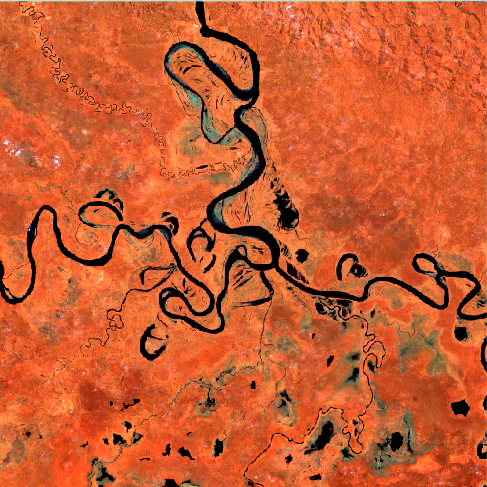
\includegraphics[height=40ex]{komposit.png}
	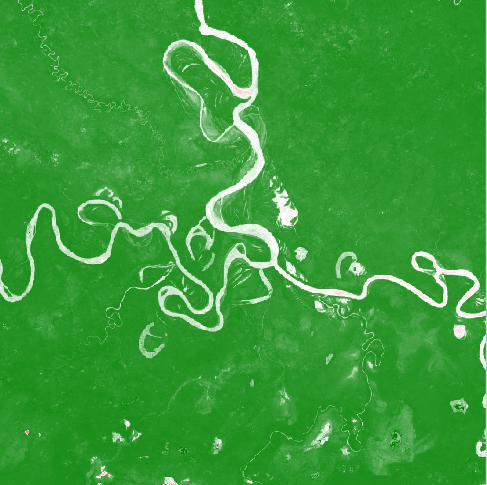
\includegraphics[height=40ex]{ndvi.png}
	\caption{NIR-SWIR1-SWIR2 composite (left) and NDVI (right) image}
\end{figure}

NIR band is used in the formula is following the spectral reflectance curve on how the interaction between multiple electomagnetic wavelength to certain object. This relation could be understand from Figure \ref{fig:spectralCurve}. Based on the curve, it can be understood that the reflectance of vegetation at its peak in NIR band wavelength interval while it have a smaller reflectance in the red spectrum while red band also have a high reflectance in soil object.

\begin{figure}[htbp]
	\label{fig:spectralCurve}
	\centering
	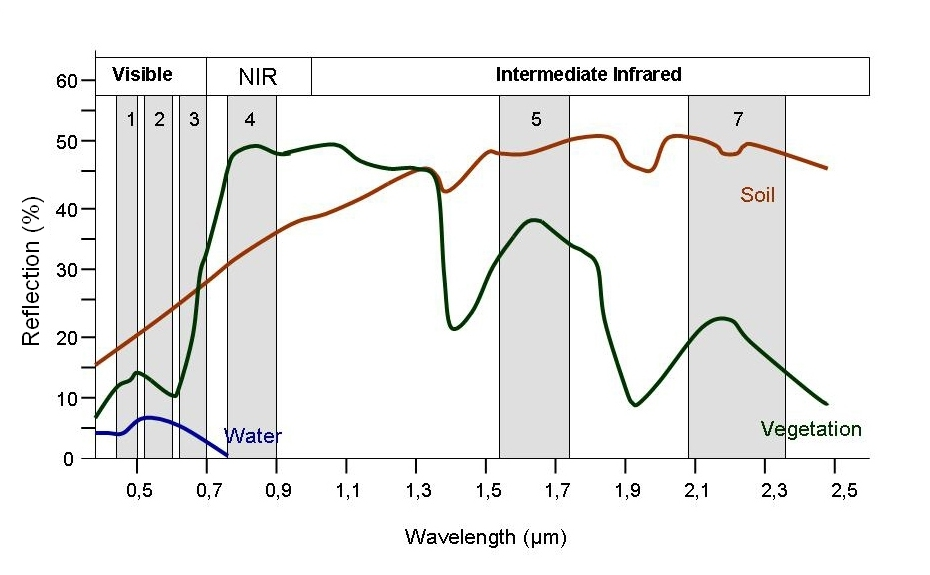
\includegraphics[width=80ex]{Reflexionskurven.jpg}
	\caption{Spectral reflectance curve of soil, vegetation, and water on multiple electromagnetic spectrum \cite{siegmund2005fernes}}
\end{figure}

While NDVI is quite famous, spectral indices is not only for vegetation. There are many spectral indices where it used for specific object and case. In indentifying built-up area, there is NDBI (Normalized Difference Built-up Index) \cite{zhang2009bi}. NDBI is using two bands: SWIR and NIR where SWIR is good enough differenciate between built-up and bareland with vegetation. NDBI is calculated using Equation \ref{eq:ndbi}. While NDBI is intended for built-up, it can also be used on purpose and not on purpose on detecting bareland, sand, and soil.

\begin{equation}
	\label{eq:ndbi}
	NIR = \frac{SWIR1 - NIR}{SWIR1 + NIR}
\end{equation}

In Landsat 8 and 9, NDBI cannot be used directly, sometime it needed additional mask. Water area usually needed to be mask first then NDBI will be applied. If that step is not covered, water could have higher NDBI value than built up like in Figure \ref{fig:ndbi}.

\begin{figure}[htbp]
	\label{fig:ndbi}
	\centering
	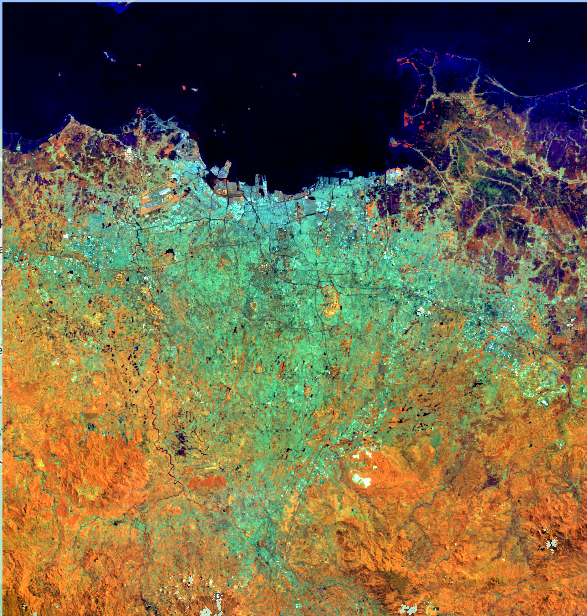
\includegraphics[width=40ex]{komposit2.png}
	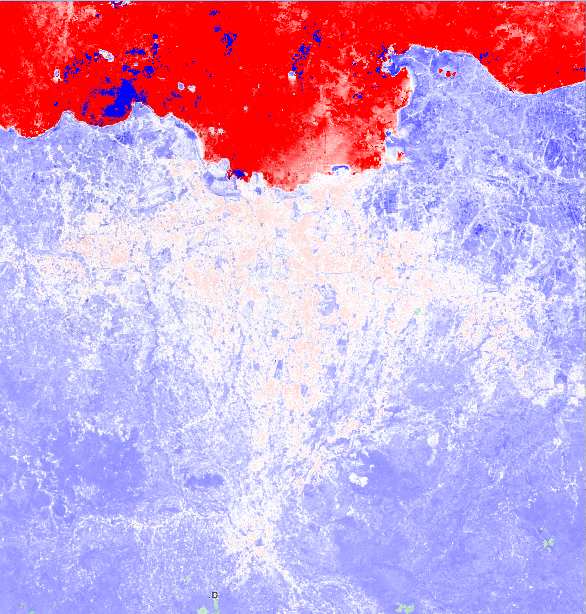
\includegraphics[width=40ex]{ndbi.png}
	\caption{Comparison of Landsat NIR-SWIR1-BLUE composite (left) and NDBI (right)}
\end{figure}

Other than NDBI, there are many more spectral indices for built-up such as Index-based Built-up Index (IBI) and New Built-up Index (NBI). For more indices, it good to follow this paper \cite{valdiviezo2018built}. The list of built-up indices mentioned in the paper can be read in Table \ref{table:urbanIndices}.

\begin{table}[htbp]
	\centering
	\caption{List of some built-up spectral indices}
	\begin{tabular}{ l  l }
		\hline

		\textbf{Indices} & \textbf{Formula} \\

		\hline

		Index-based Built-up Index & $IBI = \frac{NDBI - (SAVI + MNDWI)/2}{NDBI - (SAVI + MNDWI)/2}$ \\

		\hline
		
		New Built-up Index & $NBI = \frac{RED * SWIR}{NIR}$ \\

		\hline

		Normalized Difference Imprevious Surface Index & $NDISI = \frac{TIR - [WI + NIR + SWIR]/3}{TIR + [WI + NIR + SWIR]/3}$ \\

		\hline

		Band Ratio for Built-up Area & $BRBA = \frac{RED}{SWIR}$ \\

		\hline

		Normalized Difference Built-up Area Index & $NDBAI = \frac{SWIR1 * SWIR2 / GREEN}{SWIR1 + SWIR2 / GREEN}$ \\

		\hline
		
		Modified Built-up Index & $MBI = \frac{SWIR2 * RED - NIR^2}{RED + NIR + SWIR2}$ \\

		\hline

		Built-up Extraction Index & $BAEI = \frac{RED + L}{GREEN + SWIR}$ \\

		\hline
	\end{tabular}
	\label{table:urbanIndices}
\end{table}


\section{Calculating built-up spectral indices in Google Earth Engine}
Google Earth Engine (GEE) is cloud-based geospatial analysis software for global scale and multitemporal data \cite{gorelick2017google}. It is allow user to do analysis online without the need for high computation resources. It is also store many remote sensing data that can be use directly. This allow professionals and academics to utilize for many project and research.

Calculating spectral indices is one method to analyze the landscape using multispectral satellite imagery. This imagery are available in the GEE, so instead of downloading the image then calculate the indices in a GIS software, is it now posibble to do it directly in the cloud. 

In GEE, an imagery or stack of multispectral imagery is represented by \verb|ee.Image| object/class. This object will have several properties such as all the bands of stacked image inside, geometry boundary, date, source, and any other properties. Using the bands available in the \verb|ee.Image|, it is possible to calculate built-up indices. It could be done using mathematical operation such as \verb|add, subtract, multiply, & divide| or using \verb|ee.Image.expression| method where it receive two arguments: the formula in quoted text/string and band map or the definition of the formula's variables. Script \ref{code:expression} show the example to calculate NDBI using Landsat imagery.

\begin{lstlisting}[language=JavaScript, label={code:expression}, caption={GEE script to calculate NDBI from Landsat 8 OLI imagery}]
// Importing landsat imagery collection surface reflectance (level 2)
var landsat8 = ee.ImageCollection("LANDSAT/LC08/C02/T1_L2");

// ee.Geometry object to filter and clip image
var roi = ee.Geometry({
  "geodesic": false,
  "type": "Polygon",
  "coordinates": [
    [
      [
        110.2833489688428,
        -7.892826204719211
      ],
      [
        110.4701165469678,
        -7.892826204719211
      ],
      [
        110.4701165469678,
        -7.697580101285619
      ],
      [
        110.2833489688428,
        -7.697580101285619
      ],
      [
        110.2833489688428,
        -7.892826204719211
      ]
    ]
  ]
});

// Cloud masking
function cloudMaskOli(image){
	var qa = image.select('QA_PIXEL');
	var dilated = 1 << 1;
	var cirrus = 1 << 2;
	var cloud = 1 << 3;
	var shadow = 1 << 4;
	var mask = qa.bitwiseAnd(dilated).eq(0)
		.and(qa.bitwiseAnd(cirrus).eq(0))
		.and(qa.bitwiseAnd(cloud).eq(0))
		.and(qa.bitwiseAnd(shadow).eq(0));
	
	return image.select(['SR_B2', 'SR_B3', 'SR_B4', 'SR_B5', 'SR_B6', 'SR_B7'], ['B2', 'B3', 'B4', 'B5', 'B6', 'B7']).updateMask(mask);
}

// Filter the imagery using boundary and date
var image = landsat8.filterBounds(roi) // Filter by region
	.filterDate('2023-01-01', '2023-12-31') // Filter by date
	.map(cloudMaskOli) // Cloud mask
	.median() // Get the first image from the collection
	.clip(roi) // Clip the image
	.multiply(0.0000275).add(-0.2);

// Band map to define the band use for calculation
var bandMap = {
	NIR: image.select('B5'),
	SWIR1: image.select('B6')
};

// Calculate NDBI
var ndbi = image.expression('NDBI = (SWIR1 - NIR) / (SWIR1 + NIR)', bandMap);

// Show NDBI to map
Map.addLayer(ndbi, { min: -1, max: 1, palette: ['blue', 'white', 'red'] }, 'NDBI');
\end{lstlisting}

\section{Modelling built-up using relational operation}
NDBI is a raster value ranged -1 to 1 where the higher value mean it could have high probability to be built-up. However sometime using one indices is not enough to determine built-up, so it need another indices to mask that. Using relational operation in GEE, we could determine the condition to decice built-up area. In GEE, relational operation can be done using \verb|lt, lte, gt, gte, eq, neq, and, or|, where each will state if our threshold is lower than (\verb|lt|) or greater than (\verb|gte|) of certain value. Script \ref{code:relational} show how to classify built-up area using relational operation which utilize some indices. It also using Landsat NIR band to mask cloud. The result can be seen in Figure \ref{fig:built}.

\begin{lstlisting}[language=JavaScript, label={code:relational}, caption={GEE Script to Classify Built-up using Relational Operation}]
// image is the landsat imagery
// Band map to define the band use for calculation
var bandMap = {
	SWIR2: image.select('B7'),
	SWIR1: image.select('B6'),
	NIR: image.select('B5'),
	GREEN: image.select('B3'),
};

// Calculate MNDWI
var mdnwi = image.expression('MNDWI = (GREEN - SWIR1) / (GREEN + SWIR1)', bandMap);

// Calculate NBR2
var nbr2 = image.expression('NBR = (SWIR1 - SWIR2) / (SWIR1 + SWIR2)', bandMap);

// Calculate NDBI
var ndbi = image.expression('NDBI = (SWIR1 - NIR) / (SWIR1 + NIR)', bandMap);

// Built-up
var built = ndbi.gt(-0.1).and(mdnwi.lt(0)).and(nbr2.lte(0.2));

// Show land cover
Map.addLayer(built.selfMask(), { palette: 'lightcoral' }, 'Built-up');
\end{lstlisting}

\begin{figure}[htbp]
	\centering
	\label{fig:built}
	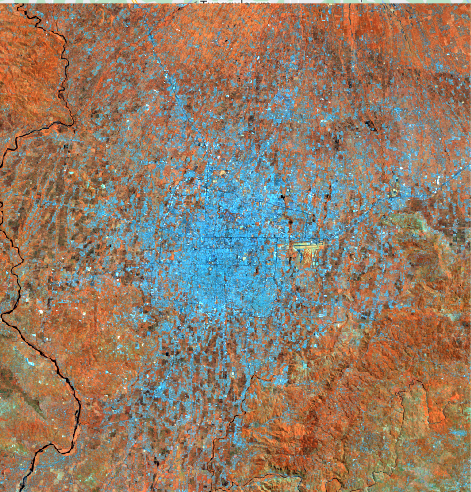
\includegraphics[width=40ex]{kompositJogja.png}
	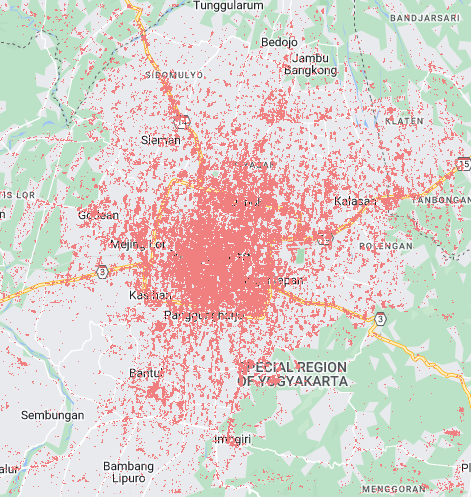
\includegraphics[width=40ex]{built.png}
	\caption{Image of Yogyakarta composite (NIR-SWIR1-SWIR2) (left) and classified built-up using spectral indices (right)}
\end{figure}

\section{Modelling urban sprawl using multitemporal data}
It is possible to model one step further using multitemporal data so that we could model how the built-up have expanded over the years. This usually need a yearly composite which will show cloud masked built-up area. Then we just stacked the multitemporal built-up area where each year have their own number assigned as urban expansion over the years. Script \ref{code:expansion} will help you to do that. The result will shown like Figure \ref{fig:expansion}.

\begin{lstlisting}[language=JavaScript, label={code:expansion}, caption={GEE Script to Model Urban Expansion}]
// Importing landsat imagery collection surface reflectance (level 2)
var landsat8 = ee.ImageCollection("LANDSAT/LC08/C02/T1_L2");
var landsat9 = ee.ImageCollection("LANDSAT/LC09/C02/T1_L2");
var landsat5 = ee.ImageCollection("LANDSAT/LT05/C02/T1_L2");
var landsat7 = ee.ImageCollection("LANDSAT/LE07/C02/T1_L2");
var landsat4 = ee.ImageCollection("LANDSAT/LT04/C02/T1_L2");

// ee.Geometry object to filter and clip image
var roi = ee.Geometry({
  "geodesic": false,
  "type": "Polygon",
  "coordinates": [
    [
      [
        110.2833489688428,
        -7.892826204719211
      ],
      [
        110.4701165469678,
        -7.892826204719211
      ],
      [
        110.4701165469678,
        -7.697580101285619
      ],
      [
        110.2833489688428,
        -7.697580101285619
      ],
      [
        110.2833489688428,
        -7.892826204719211
      ]
    ]
  ]
});

// Year list to map
var yearList = [1990, 1995, 2000, 2005, 2010, 2015, 2020];

// Function to filter
function filterCol(col, roi, date){
	return col.filterDate(date[0], date[1]).filterBounds(roi);
}

// Composite function
function landsat457(roi, date){
	var col = filterCol(landsat4, roi, date).merge(filterCol(landsat5, roi, date)).merge(filterCol(landsat7, roi, date));
	var image = col.map(cloudMaskTm).median().clip(roi);
	return image;
}

function landsat89(roi, date){
	var col = filterCol(landsat8, roi, date).merge(filterCol(landsat9, roi, date));
	var image = col.map(cloudMaskOli).median().clip(roi);
	return image;
}

// Cloud mask
function cloudMaskTm(image){
	var qa = image.select('QA_PIXEL');
	var dilated = 1 << 1;
	var cloud = 1 << 3;
	var shadow = 1 << 4;
	var mask = qa.bitwiseAnd(dilated).eq(0)
		.and(qa.bitwiseAnd(cloud).eq(0))
		.and(qa.bitwiseAnd(shadow).eq(0));
	
	return image.select(['SR_B1', 'SR_B2', 'SR_B3', 'SR_B4', 'SR_B5', 'SR_B7'], ['B2', 'B3', 'B4', 'B5', 'B6', 'B7']).updateMask(mask);
}

function cloudMaskOli(image){
	var qa = image.select('QA_PIXEL');
	var dilated = 1 << 1;
	var cirrus = 1 << 2;
	var cloud = 1 << 3;
	var shadow = 1 << 4;
	var mask = qa.bitwiseAnd(dilated).eq(0)
		.and(qa.bitwiseAnd(cirrus).eq(0))
		.and(qa.bitwiseAnd(cloud).eq(0))
		.and(qa.bitwiseAnd(shadow).eq(0));
	
	return image.select(['SR_B2', 'SR_B3', 'SR_B4', 'SR_B5', 'SR_B6', 'SR_B7'], ['B2', 'B3', 'B4', 'B5', 'B6', 'B7']).updateMask(mask);
}

// Generate image per year
var builtCol = ee.ImageCollection(yearList.map(function(year){
	var start = ee.Date.fromYMD(year, 1, 1);
	var end = ee.Date.fromYMD(year, 12, 31);
	var date = [start, end];
	
	// Conditional on landsat collection to use
	var landsat;
	if (year < 2014) {
		landsat = landsat457;
	} else {
		landsat = landsat89;
	}
	
	// Create an image composite
	var image = landsat(roi, date).multiply(0.0000275).add(-0.2);
	
	// Show the image
	Map.addLayer(image, { min: [0.1, 0.05, 0.025], max: [0.4, 0.3, 0.2], bands: ['B5', 'B6', 'B7'] }, 'Landsat_' + year, false);
	
	// Band map
	var bandMap = { 
		NIR: image.select('B5'), 
		SWIR: image.select('B6'), 
		RED: image.select('B4'), 
		GREEN: image.select('B3'), 
		BLUE: image.select('B2') 
	};
	
	// Normalized Difference Built-up Index
	var ndbi = image.expression('(SWIR - NIR) / (SWIR + NIR)', bandMap).rename('NDBI');
	
	// Show the NDBI
	Map.addLayer(ndbi, { min: -1, max: 1, palette: ['blue', 'white', 'red'] }, 'NDBI_' + year, false);
	
	// Modified Normalized Difference Water Index
	var mndwi = image.expression('(GREEN - SWIR) / (GREEN + SWIR)', bandMap).rename('MNDWI');
	
	// Show the MNDWI
	Map.addLayer(mndwi, { min: -1, max: 1, palette: ['red', 'white', 'blue'] }, 'MNDWI_' + year, false);
	
	// Built up
	var built = ee.Image(0).where(ndbi.gt(-0.1).and(mndwi.lte(0)), year)
		.selfMask()
		.clip(roi);
	Map.addLayer(built, { palette: 'lightcoral' }, 'Built-up_' + year, false);
	
	// Image area for calculation
	var area = built.multiply(ee.Image.pixelArea().multiply(0.0001)).rename('area');
	
	return built.toUint16().rename('built').addBands(area).set('year', year, 'system:time_start', start);
}));

// Create dictionary for each year expansion for visualization
var dict = {
	'built_class_values': yearList,
	'built_class_palette': ['800080', '0000FF', '00FFFF', '008000', 'FFFF00', 'FFA500', 'FF0000']
};

// Create expansion image
var urbanExpansion = builtCol.select('built').min().set(dict);
Map.addLayer(urbanExpansion, {}, 'Urban_expansion');

// Create legend for expansion year
var legend = ui.Panel([ui.Label('Urban expansion')], ui.Panel.Layout.flow('vertical'), { position: 'bottom-left' });
yearList.map(function(year, index){
	legend.add(ui.Panel([
		ui.Label('', { width: '20px', height: '20px', backgroundColor: dict.built_class_palette[index], border: '0.5px solid black' }),
		ui.Label(year)
	], ui.Panel.Layout.flow('horizontal')));
});
Map.add(legend);

// Create table to show the urban area change
var areaChart = ui.Chart.image.series(builtCol.select('area'), roi, ee.Reducer.sum(), 30, 'year')
	.setChartType('AreaChart')
	.setOptions({
		title: 'Urban area (Ha)',
		hAxis: { title: 'Year' },
		vAxis: { title: 'Area (Ha)' }
	});
print(areaChart);
\end{lstlisting}

\begin{figure}[htbp]
	\centering
	\label{fig:expansion}
	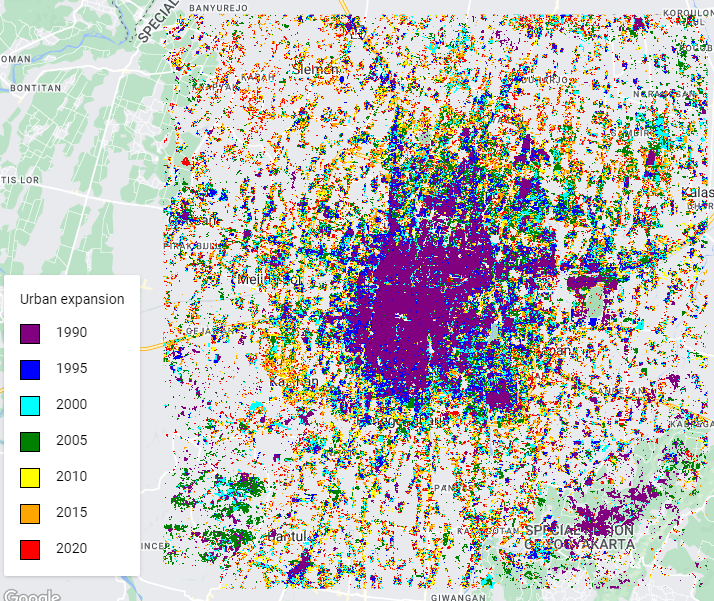
\includegraphics[width=40ex]{urbanExpansion.png}
	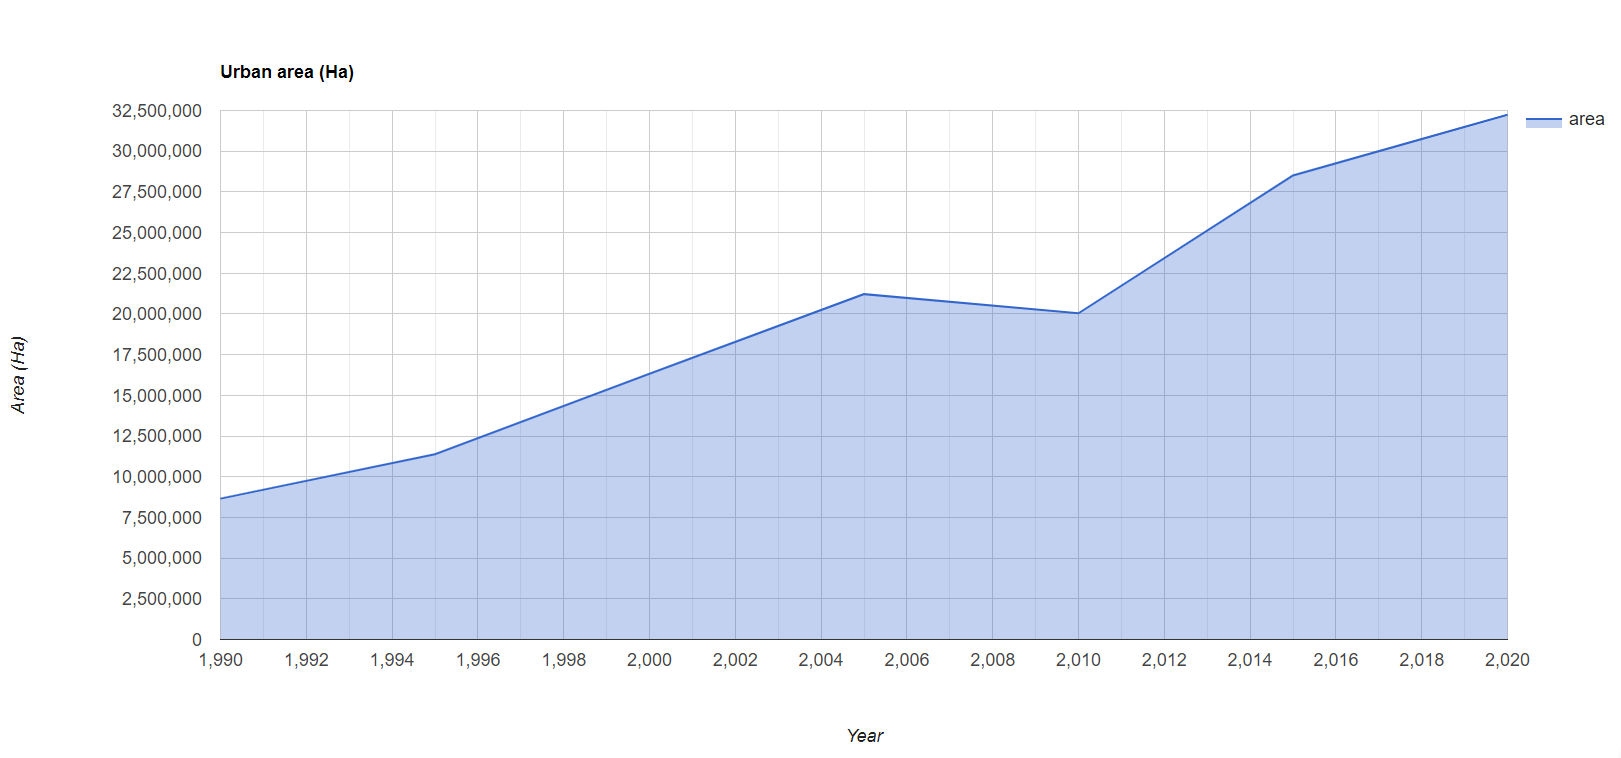
\includegraphics[width=50ex]{urbanArea.png}
	\caption{Urban expansion area by year (left) and the area changes (right)}
\end{figure}

\section{Introducing Land Surface Temperature (LST) and land cover}
Land surface temperature (LST) is the temperature generated when the energy from the sun hit the surface of the earth when touched. It is different than air temperature like in weather news. LST can be retrieved using thermal infared wavelength in multispectral imagery like in Landsat and MODIS. LST have high correlation with the object on the surface of the Earth. Usually greener and wet object have lower LST than dry and barren land although another factor such as climate and atmospheric difference also affected it.

Usind NDVI, the LST usually high in range 0 - 0.3 and keep decreasing the further away from that range as seen in Figure \ref{fig:ndviLst}. It is due the characteristic of vegetation and water that absorb thermal infrared more than bareland. Using this model, we can model what will happen to LST in the future.

\begin{figure}[htbp]
	\label{fig:ndviLst}
	\centering
	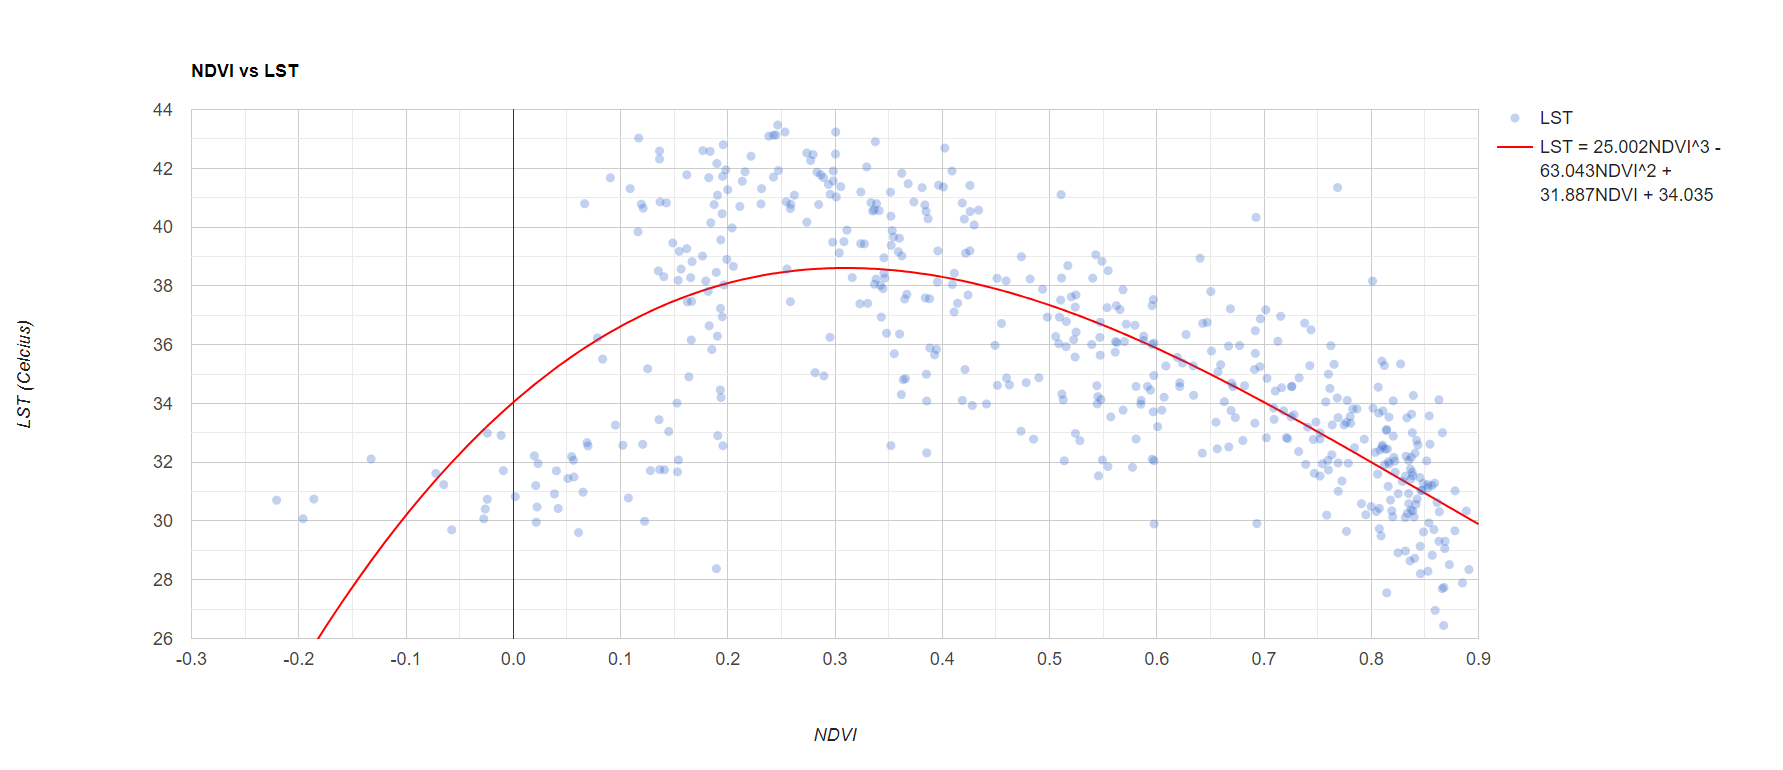
\includegraphics[width=90ex]{ndviLst.png}
	\caption{Relationsip between NDVI and LST}
\end{figure}

\section{Compositing and preprocessing LST data}
There are two ways of generating LST data from Landsat: using the surface temperature ready band in level 2 collection or calculate yourself from the raw digital number data using known formula. To use ready to use data, you can select band \verb|ST_B10| in the collection then multiply it by 0.00341802 and add 149 to turn it up into Kelvin like in Script \ref{code:lstReady}. It will show LST like in Figure \ref{fig:lstReady}.

\begin{lstlisting}[language=JavaScript, label={code:lstReady}, caption={GEE Script get LST data}]
// Importing landsat imagery collection surface reflectance (level 2)
var landsat8 = ee.ImageCollection("LANDSAT/LC08/C02/T1_L2");

// ee.Geometry object to filter and clip image
var roi = ee.Geometry({
	"geodesic": false,
	"type": "Polygon",
	"coordinates": [
		[
			[
				110.2833489688428,
				-7.892826204719211
			],
			[
				110.4701165469678,
				-7.892826204719211
			],
			[
				110.4701165469678,
				-7.697580101285619
			],
			[
				110.2833489688428,
				-7.697580101285619
			],
			[
				110.2833489688428,
				-7.892826204719211
			]
		]
	]
});

// Cloud mask
function cloudMaskOli(image){
  var qa = image.select('QA_PIXEL');
  var dilated = 1 << 1;
  var cirrus = 1 << 2;
  var cloud = 1 << 3;
  var shadow = 1 << 4;
  var mask = qa.bitwiseAnd(dilated).eq(0)
    .and(qa.bitwiseAnd(cirrus).eq(0))
    .and(qa.bitwiseAnd(cloud).eq(0))
    .and(qa.bitwiseAnd(shadow).eq(0));
  
  return image.select(['SR_B2', 'SR_B3', 'SR_B4', 'SR_B5', 'SR_B6', 'SR_B7'], ['B2', 'B3', 'B4', 'B5', 'B6', 'B7'])
    .multiply(0.0000275).add(-0.2)
    .addBands(image.select(['ST_B10'], ['LST']).multiply(0.00341802).add(149).add(-273.15))
    .updateMask(mask);
}

// Image composte
var image = landsat8.filterBounds(roi).filterDate('2022-01-01', '2022-12-31').map(cloudMaskOli).median().clip(roi);

// Show LST
Map.addLayer(image, { min: 30, max: 40, palette: ['black', 'purple', 'blue', 'cyan', 'green', 'yellow', 'red'], bands: 'LST' }, 'LST');

// Calcualte NDVI
var bandMap = {
  NIR: image.select('B5'),
  RED: image.select('B4'),
  SWIR1: image.select('B6'),
  SWIR2: image.select('B7'),
  GREEN: image.select('B3')
};

// NDVI group
var groupNdvi = ee.Image(0).where(ndvi.lte(0), 1)
  .where(ndvi.gt(0).and(ndvi.lte(0.2)), 1)
  .where(ndvi.gt(0.2).and(ndvi.lte(0.4)), 2)
  .where(ndvi.gt(0.4).and(ndvi.lte(0.6)), 3)
  .where(ndvi.gt(0.6).and(ndvi.lte(0.8)), 4)
  .where(ndvi.gt(0.8), 5)
  .selfMask()
  .rename('group');
\end{lstlisting}

\begin{figure}[htbp]
	\label{fig:lstReady}
	\centering
	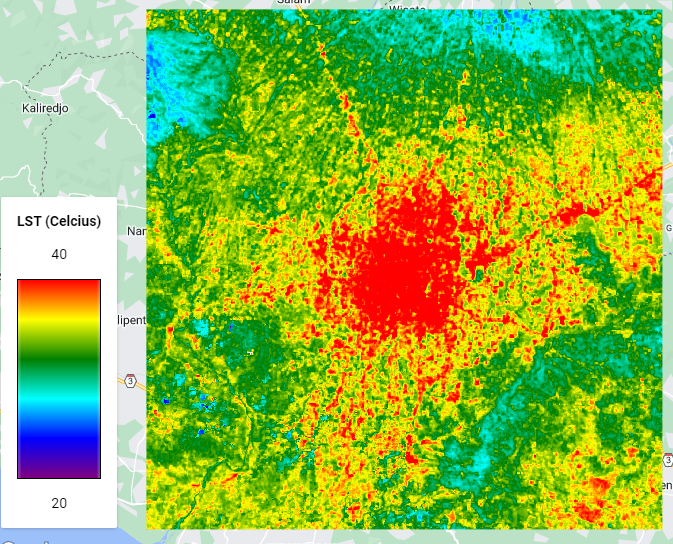
\includegraphics[width=80ex]{lstReady.png}
	\caption{LST generated from Landsat 8 Level 2}
\end{figure}

If you want to calculate LST yourself you could use Mono-window algorithm, Split-window algorithm, Planck, and many more. To do it you can follow Script \ref{code:lstProcess}. The result will be LST raster data like Figure \ref{fig:lstMany}.

\begin{lstlisting}[language=JavaScript, label={code:lstProcess}, caption={GEE Script to calculate LST manually}]
// Calculate LST manually
// TOA to radiance
function toaRadiance(image){
	var L10 = image.expression('(M * Q) + A', {
		M: ee.Number(image.get('RADIANCE_MULT_BAND_10')),
		Q: image.select('B10'),
		A: ee.Number(image.get('RADIANCE_ADD_BAND_10'))
	}).rename('B10_Rad');
	
	var L11 = image.expression('(M * Q) + A', {
		M: ee.Number(image.get('RADIANCE_MULT_BAND_11')),
		Q: image.select('B11'),
		A: ee.Number(image.get('RADIANCE_ADD_BAND_11'))
	}).rename('B11_Rad');
	
	return image.addBands([L10, L11]);
}

// TOA to brightness temperature
function toaBrightnessTemp(image){
		var T10 = image.expression('K2 / (log((K1 / L) + 1))', {
		K1: ee.Number(image.get('K1_CONSTANT_BAND_10')),
		K2: ee.Number(image.get('K2_CONSTANT_BAND_10')),
		L: image.select('B10_Rad')
	}).rename('B10_BT');
	
		var T11 = image.expression('K2 / (log((K1 / L) + 1))', {
		K1: ee.Number(image.get('K1_CONSTANT_BAND_11')),
		K2: ee.Number(image.get('K2_CONSTANT_BAND_11')),
		L: image.select('B11_Rad')
	}).rename('B11_BT');
	
	
	return image.addBands([T10, T11]);
}

// Landsat 8 raw
var landsat8raw = ee.ImageCollection('LANDSAT/LC08/C02/T1').filterBounds(roi).filterDate('2022-01-01', '2022-12-31');

// Landsat 8 LST
var landsat8Lst = landsat8raw.map(function(image){
	// Cloud masking
	var qa = image.select('QA_PIXEL');
	var dilated = 1 << 1;
	var cirrus = 1 << 2;
	var cloud = 1 << 3;
	var shadow = 1 << 4;
	var mask = qa.bitwiseAnd(dilated).eq(0)
		.and(qa.bitwiseAnd(cirrus).eq(0))
		.and(qa.bitwiseAnd(cloud).eq(0))
		.and(qa.bitwiseAnd(shadow).eq(0));
	
	image = image.updateMask(mask);
	
	// Toa radiance
	image = toaRadiance(image);
	
	// Toa brightness
	image = toaBrightnessTemp(image);
	
	// MWA
	var mwa = image.expression('((ai * (1 - Ci - Di)) + (((bi * (1 - Ci - Di)) + Ci + Di) * Ti) - (Di * Ta)) / Ci', {
		ai: -67.355351,
		bi: 0.458606,
		Ci: 0.98 * 0.9,
		Di: image.expression('(1 - ti) * (1 + ((1 + 0.98) * ti))', { ti: 0.95 }),
		Ti: image.select('B10_BT'),
		Ta: 288
	}).add(-273.15).rename('MWA');
	
	// SWA
	var swa = image.expression('B10 + (2.946 * (B10 - B11)) - 0.038', {
		B10: image.select('B10_BT'),
		B11: image.select('B11_BT')
	}).add(-273.15).rename('SWA');
	
	// Plank
	var planck = image.expression('(BT / (1 + (((A * BT) / p) * log(EMIT))))', {
		BT: image.select('B10_BT'),
		A: 10.895,
		p: 1438 * 10000,
		EMIT: 249.9
	}).add(-273.15).rename('Planck');
	
	return ee.Image([mwa, swa, planck]);
}).median().clip(roi);

// LST palette
var lstPalette = ['purple', 'blue', 'cyan', 'green', 'yellow', 'red'];
Map.addLayer(landsat8Lst.select('MWA'), { min: 20, max: 40, palette: lstPalette }, 'LST MWA');
Map.addLayer(landsat8Lst.select('SWA'), { min: 20, max: 40, palette: lstPalette }, 'LST SWA');
Map.addLayer(landsat8Lst.select('Planck'), { min: 20, max: 40, palette: lstPalette }, 'LST Planck');
\end{lstlisting}

\begin{figure}
	\label{fig:lstMany}
	\centering
	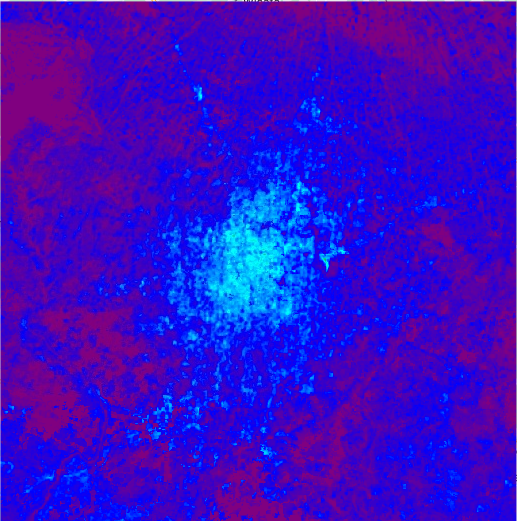
\includegraphics[width=30ex]{lstMwa.png}
	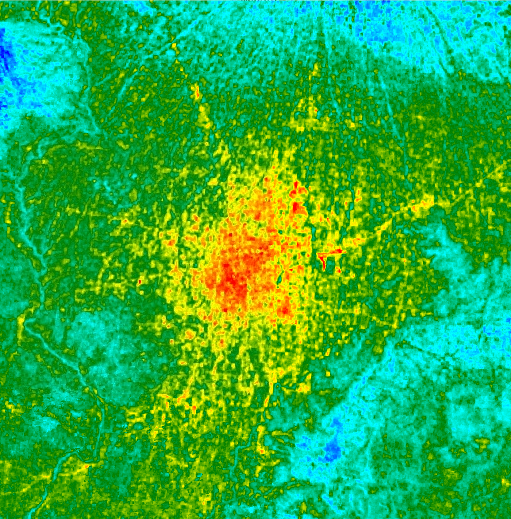
\includegraphics[width=30ex]{lstSwa.png}
	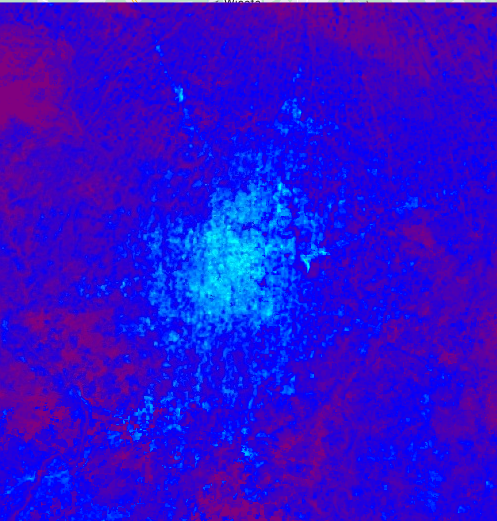
\includegraphics[width=30ex]{lstPlanck.png}
	\caption{LST with multiple algorithms: MWA (left), SWA (center), and Planck (right)}
\end{figure}

\section{Modelling LST and urban density data}
We can see the relationship between LST and NDVI but it is also possible to model it using urban density. Urban density index is how dense a built-up area which can be calculated using built-up and its neigborhood average built-up area. Urban density can be generated using convolution or focal operation of built-up area. In GEE, we can utilize \verb|reduceNeighborhood| or \verb|focalMean, focalMode, focalMedian, focalMax, and focalMin| where it will use \verb|ee.Kernel| as the window. To generate urban density index and model it with LST you can follow Script \ref{code:urbanDensity}. Urban density will look like Figure \ref{fig:urbanDensity}.

\begin{lstlisting}[language=JavaScript, label={code:urbanDensity}, caption={GEE Script to model urban density and LST}]
// Sample for chart
var sample = image.addBands([ndvi, groupNdvi]).stratifiedSample({
	numPoints: 100,
	region: roi,
	scale: 30,
	classBand: 'group'
});

// Chart LST and NDVI
var chart = ui.Chart.feature.byFeature(sample, 'NDVI', ['LST'])
	.setChartType('ScatterChart')
	.setOptions({
		title: 'NDVI vs LST',
		dataOpacity: 0.3,
		hAxis: {
			title: 'NDVI'
		},
		vAxis: {
			title: 'LST (Celcius)'
		},
		trendlines: {
			0: {
				type: 'polynomial',
				opacity: 1,
				color: 'red',
				visibleInLegend: true,
			}
		}
	});
print(chart);

// MDNWI
var mndwi = image.expression('MNDWI = (GREEN - SWIR2) / (GREEN + SWIR2)', bandMap);
Map.addLayer(mndwi, { min: -1, max: 1, palette: ['red', 'white', 'blue']}, 'MNDWI', false);

// NDBI
var ndbi = image.expression('NDBI = (SWIR2 - NIR) / (SWIR2 + NIR)', bandMap);
Map.addLayer(ndbi, { min: -1, max: 1, palette: ['blue', 'white', 'red']}, 'NDBI', false);

// NBR2
var nbr2 = image.expression('NBR2 = (SWIR1 - SWIR2) / (SWIR1 + SWIR2)', bandMap);
Map.addLayer(nbr2, { min: -1, max: 1, palette: ['red', 'white', 'green']}, 'NBR2', false);

// Built-up
var built = mndwi.lte(0).and(ndbi.gte(-0.5));
Map.addLayer(built.selfMask(), { palette: 'lightcoral' }, 'Built', false);

// Urban density
var urbanDensity = built.focalMean(3).reproject('EPSG:4326', null, 30).rename('urban_density');
Map.addLayer(urbanDensity, { min: 0, max: 1, palette: lstPalette }, 'Urban density');

// Sample
var sampleDensity = ee.Image([image.select('LST'), urbanDensity, groupNdvi]).stratifiedSample({
	numPoints: 200,
	classBand: 'group',
	scale: 30,
	region: roi
}).randomColumn();
Map.add(legendGradient('Urban density index', { min: 0, max: 1, palette: lstPalette}, 'bottom-right'));

// Chart
var chartDensity = ui.Chart.feature.byFeature(sampleDensity, 'urban_density', ['LST'])
	.setChartType('ScatterChart')
	.setOptions({
		title: 'Urban density vs LST',
		dataOpacity: 0.3,
		hAxis: {
			title: 'Urban density'
		},
		vAxis: {
			title: 'LST (Celcius)'
		},
		trendlines: {
			0: {
				type: 'linear',
				opacity: 1,
				color: 'red',
				visibleInLegend: true,
			}
		}
	});
print(chartDensity);

// Split sample to train and test
var train = sampleDensity.filter(ee.Filter.lte('random', 0.8));
var test = sampleDensity.filter(ee.Filter.gt('random', 0.8));

// Linear regression model
var model = train.reduceColumns(ee.Reducer.linearFit(), ['urban_density', 'LST']);
var scale = ee.Number(model.get('scale'));
var offset = ee.Number(model.get('offset'));

// Test model
var cm = test.map(function(feat){
	var lst = ee.Number(feat.get('urban_density'))
		.multiply(scale)
		.add(offset);
	return feat.set('prediction', lst);
});

// Accuracy
var chartAccuracy = ui.Chart.feature.byFeature(cm, 'LST', ['prediction'])
	.setChartType('ScatterChart')
	.setOptions({
		title: 'LST reference vs prediction (Celcius)',
		dataOpacity: 0.3,
		hAxis: {
			title: 'Reference'
		},
		vAxis: {
			title: 'Prediction'
		},
		trendlines: {
			0: {
				type: 'linear',
				opacity: 1,
				color: 'red',
				visibleInLegend: true,
				showR2: true
			}
		}
	});
print(chartAccuracy);

// Apply model
var lstPrediction = urbanDensity.multiply(scale).add(offset);
Map.addLayer(lstPrediction, { min: 20, max: 40, palette: lstPalette }, 'LST prediction from urban density');
\end{lstlisting}

In the script, we try to do linear regression between LST and urban density index, the result shows that it have high correlation at Figure \ref{fig:lstUrbanDensityCorrelation}. If we apply the regression, we will have $R^2$ 0.685 at Figure \ref{fig:lstUrbanDensityAccuracy}. Comparison between reference and prediction LST can be seen in \ref{fig:lstReferenceVsPrediction}.

\begin{figure}
	\label{fig:urbanDensity}
	\centering
	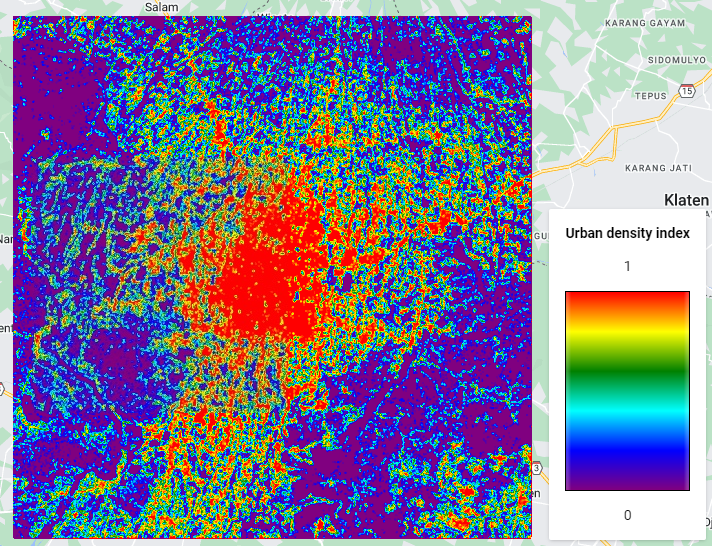
\includegraphics[width=80ex]{urbanDensity.png}
	\caption{Urban density index}
\end{figure}

\begin{figure}[htbp]
	\label{fig:lstUrbanDensityCorrelation}
	\centering
	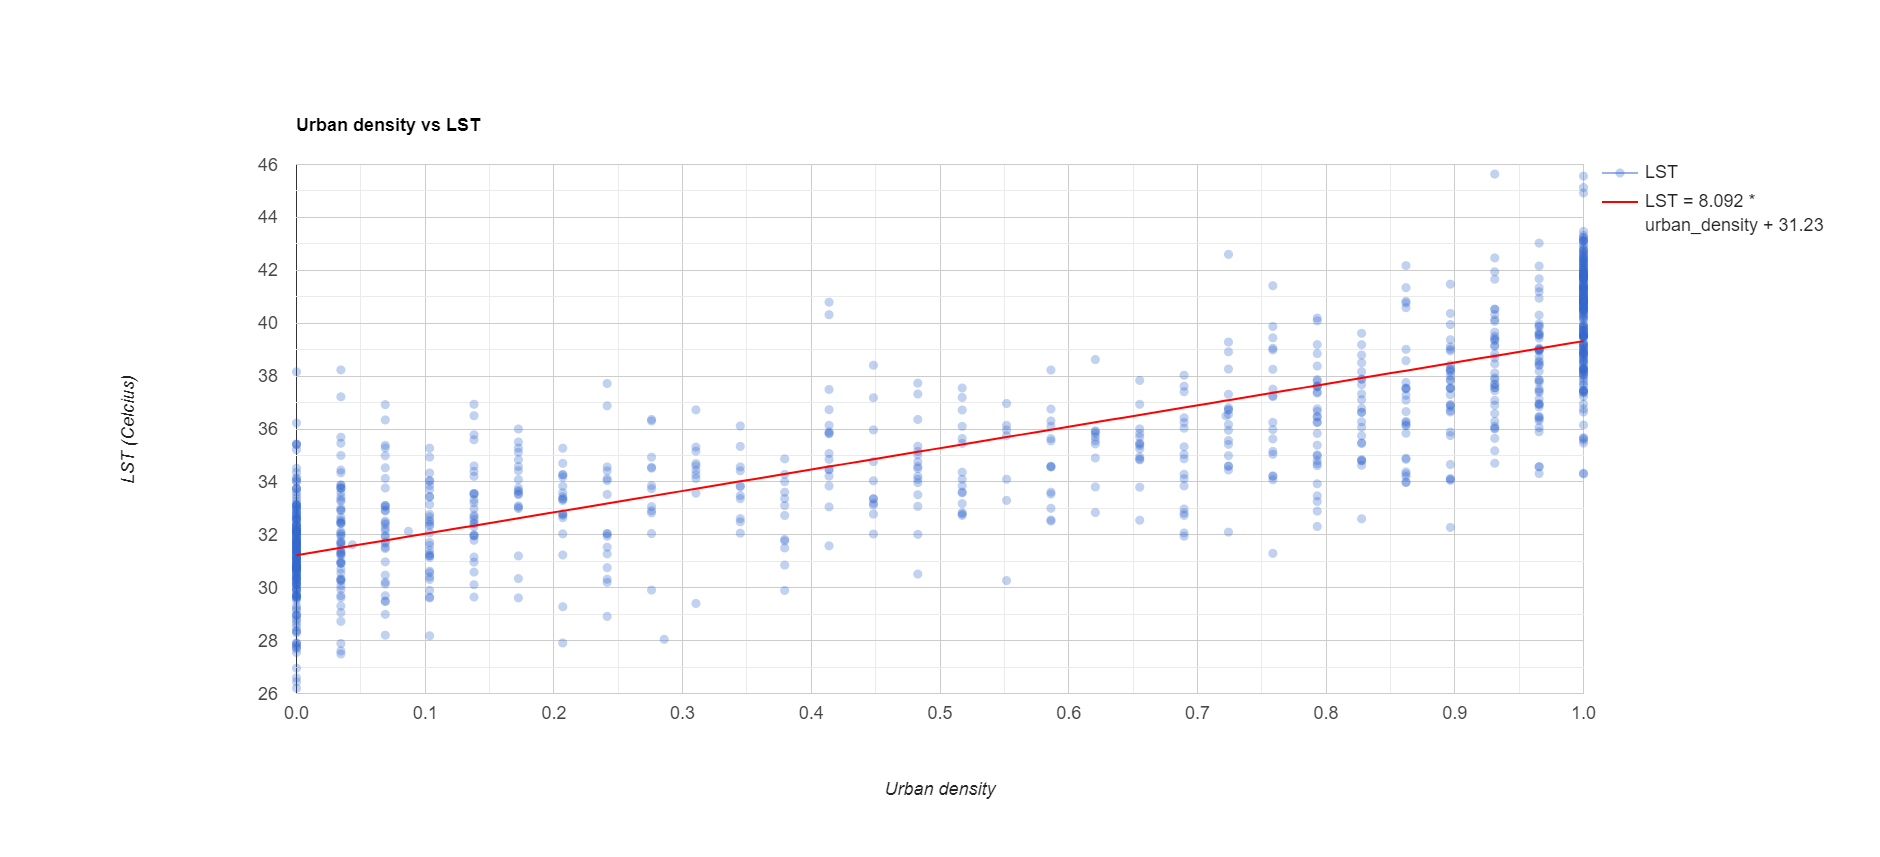
\includegraphics[width=90ex]{urbanDensityLstChart.png}
	\caption{Correlation between LST and urban density index}
\end{figure}

\begin{figure}[htbp]
	\label{fig:lstUrbanDensityAccuracy}
	\centering
	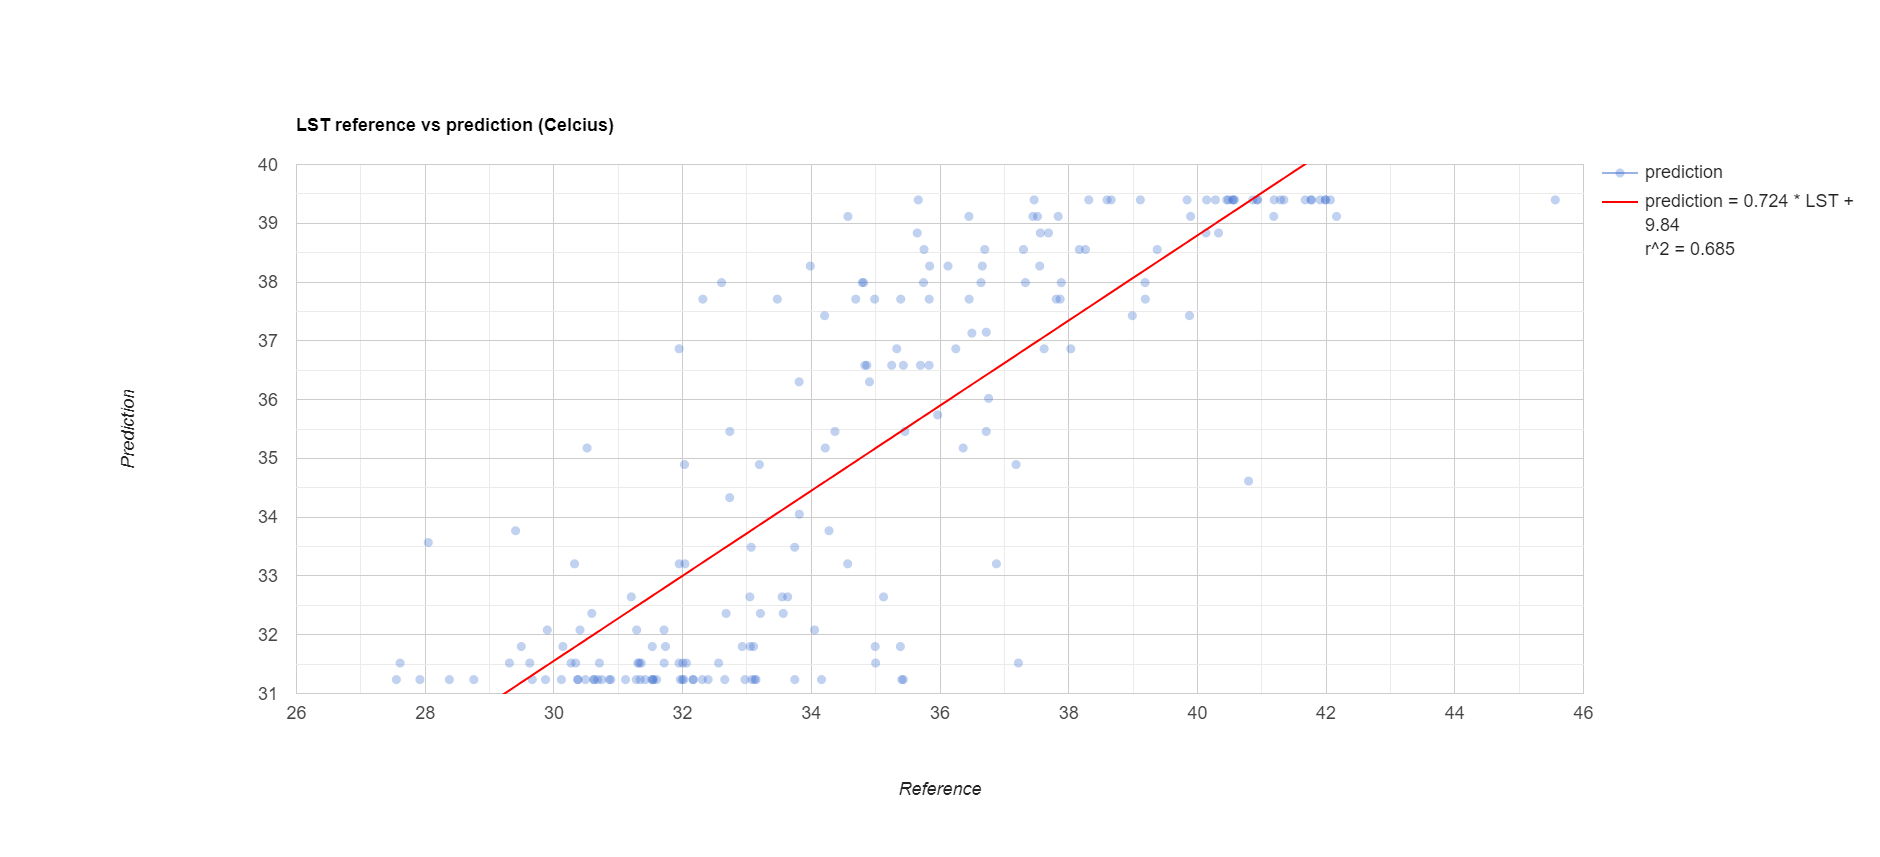
\includegraphics[width=90ex]{accuracyLstUrbanDensity.png}
	\caption{Regression accuracy using urban density index to predict LST}
\end{figure}

\begin{figure}[htbp]
	\label{fig:lstReferenceVsPrediction}
	\centering
	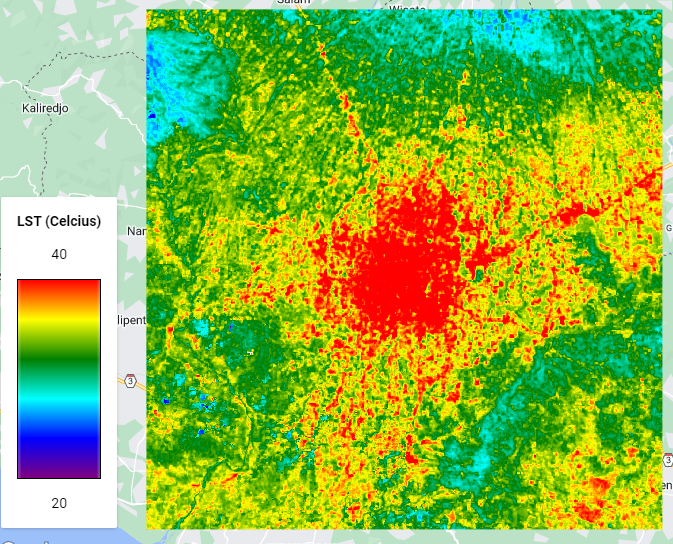
\includegraphics[width=40ex]{lstReady.png}
	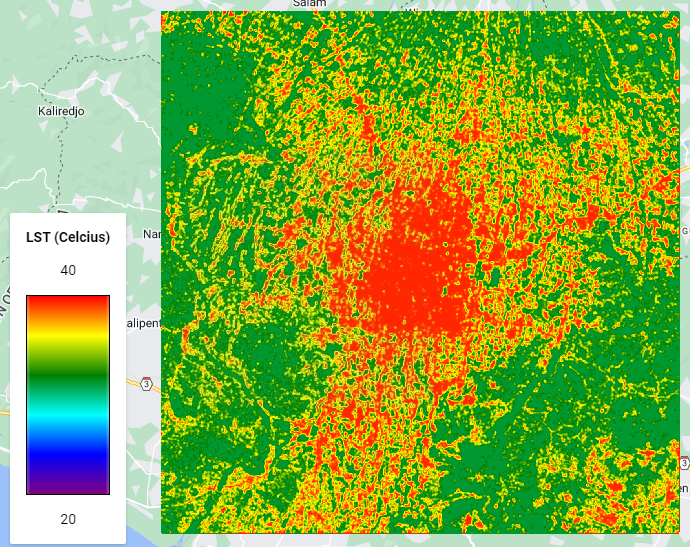
\includegraphics[width=40ex]{lstPrediction.png}
	\caption{LST reference (left) vs prediction (right)}
\end{figure}

\section{Predict future LST using machine learning}
Able to predict LST using built-up and bareland land cover mean it is also possible to predict LST in the future too. It also possible to add another variables such as elevation and other land cover density. In this part, I will show you how to predict LST in 2023 using data from 2021 and 2022. Then, we compare the result to 2023. You can follow the Script \ref{code:futureLst}.


\begin{lstlisting}[language=JavaScript, label={code:futureLst}, caption={GEE Script to predict future LST}]
// Importing landsat imagery collection surface reflectance (level 2)
var landsat8 = ee.ImageCollection("LANDSAT/LC08/C02/T1_L2");

// ee.Geometry object to filter and clip image
var roi = ee.Geometry({
	"geodesic": false,
	"type": "Polygon",
	"coordinates": [
		[
			[
				110.2833489688428,
				-7.892826204719211
			],
			[
				110.4701165469678,
				-7.892826204719211
			],
			[
				110.4701165469678,
				-7.697580101285619
			],
			[
				110.2833489688428,
				-7.697580101285619
			],
			[
				110.2833489688428,
				-7.892826204719211
			]
		]
	]
});

// Predict future built-up bareland
// Years data for prediction
var years = [2021, 2022, 2023];
var yearToPredict = 2023;

// Elevation data
var srtm = ee.Image("USGS/SRTMGL1_003").clip(roi);

// Years image
var images = years.map(function(year){
	var image = landsat8.filterBounds(roi).filterDate(year + '-01-01', year + '-12-31').map(cloudMaskOli).median().clip(roi);
	
	// Band map
	var bandMap = {
		NIR: image.select('B5'),
		RED: image.select('B4'),
		SWIR1: image.select('B6'),
		SWIR2: image.select('B7'),
		GREEN: image.select('B3')
	};
	
	// MDNWI
	var mndwi = image.expression('MNDWI = (GREEN - SWIR2) / (GREEN + SWIR2)', bandMap);
	//Map.addLayer(mndwi, { min: -1, max: 1, palette: ['red', 'white', 'blue']}, 'MNDWI_' + year, false);
	
	// NDBI
	var ndbi = image.expression('NDBI = (SWIR2 - NIR) / (SWIR2 + NIR)', bandMap);
	//Map.addLayer(ndbi, { min: -1, max: 1, palette: ['blue', 'white', 'red']}, 'NDBI_' + year, false);
	
	// NBR2
	var nbr2 = image.expression('NBR2 = (SWIR1 - SWIR2) / (SWIR1 + SWIR2)', bandMap);
	//Map.addLayer(nbr2, { min: -1, max: 1, palette: ['red', 'white', 'green']}, 'NBR2_' + year, false);
	
	// NBR
	var nbr = image.expression('NBR = (NIR - SWIR2) / (NIR + SWIR2)', bandMap);
	//Map.addLayer(nbr, { min: -1, max: 1, palette: ['red', 'white', 'green']}, 'NBR_' + year, false);
	
	// Built-up
	var built = mndwi.lte(0).and(ndbi.gte(-0.5)).and(nbr.lte(0.2)).rename('built');
	//Map.addLayer(built, { palette: 'lightcoral' }, 'Built_' + year, false);
	
	// Water
	var water = mndwi.gt(0.1).rename('water');
	//Map.addLayer(water, { palette: 'lightskyblue' }, 'Water_' + year, false);
	
	// Sparse vegetation
	var sparseVegetation = nbr.gt(0.3).and(nbr.lt(0.6)).rename('sparse_vegetation');
	//Map.addLayer(sparseVegetation, { palette: 'lightgreen' }, 'SparseVegetation_' + year, false);
	
	// Sparse vegetation
	var denseVegetation = nbr.gt(0.6).rename('dense_vegetation');
	//Map.addLayer(denseVegetation, { palette: 'darkgreen' }, 'DenseVegetation_' + year, false);
	
	// Bareland
	var bareland =  mndwi.lte(0).and(ndbi.gte(-0.5)).and(nbr2.gt(0.2)).and(nbr.lte(0.3)).rename('bareland');
	//Map.addLayer(bareland, { palette: 'burlywood' }, 'Bareland_' + year, false);

	
	return ee.Image([built, water, sparseVegetation, denseVegetation, bareland, image.select('LST')]);
});

// Images
var image2021 = images[0];
var image2022 = images[1];

// predictors
var predictors = ['built', 'bareland', 'water', 'sparse_vegetation', 'dense_vegetation', 'elevation', 'LST_first'];
var label = 'LST_last';

// Sample
var samplePredictionLst = ee.Image([
	image2021.addBands(srtm).select(
		['built', 'bareland', 'water', 'sparse_vegetation', 'dense_vegetation', 'elevation', 'LST'], 
		predictors
	),
	image2022.select(['LST'], ['LST_last']),
	groupNdvi
]).stratifiedSample({
	numPoints: 200,
	scale: 30,
	classBand: 'group',
	region: roi
}).randomColumn();

// Split into train and testing
var trainLst = samplePredictionLst.filter(ee.Filter.lte('random', 0.8));
var testLst = samplePredictionLst.filter(ee.Filter.gt('random', 0.8));

// Model
var modelLst = ee.Classifier.smileRandomForest(50).train(trainLst, label, predictors)
	.setOutputMode('REGRESSION');
print(modelLst.explain());

// Apply amodel to 2022 to predict 2023
var lst2023Prediction = image2022.addBands(srtm)
	.select(
		['built', 'bareland', 'water', 'sparse_vegetation', 'dense_vegetation', 'elevation', 'LST'],
		predictors
	).classify(modelLst, 'LST_prediction_2023');
Map.addLayer(lst2023Prediction, { min: 20, max: 40, palette: lstPalette }, 'LST prediction 2023', false);

// LST truth 2023
var lstTruth2023 = images[2].select(['LST'], ['LST_truth_2023']);
Map.addLayer(lstTruth2023, { min: 20, max: 40, palette: lstPalette }, 'LST reference 2023', false);

// Accuracy assessment
var lstAssessment = ee.Image([lstTruth2023, lst2023Prediction, groupNdvi]).stratifiedSample({
	region: roi,
	scale: 30,
	classBand: 'group',
	numPoints: 200
});

// Chart
var lstChartPrediction = ui.Chart.feature.byFeature(lstAssessment, 'LST_truth_2023', ['LST_prediction_2023'])
	.setChartType('ScatterChart')
	.setOptions({
		title: 'LST reference vs prediction (Celcius) in 2023',
		dataOpacity: 0.3,
		hAxis: {
			title: 'Reference'
		},
		vAxis: {
			title: 'Prediction'
		},
		trendlines: {
			0: {
				type: 'linear',
				opacity: 1,
				color: 'red',
				visibleInLegend: true,
				showR2: true
			}
		}
	});
print(lstChartPrediction);
\end{lstlisting}
	
	After we predict the future LST in 2023, we can compare it with truth in 2023. Figure \ref{fig:lst2023} show 1 on 1 comparison while \ref{fig:r22023} show how accurate our prediction.
	
\begin{figure}[htbp]
	\label{fig:lst2023}
	\centering
	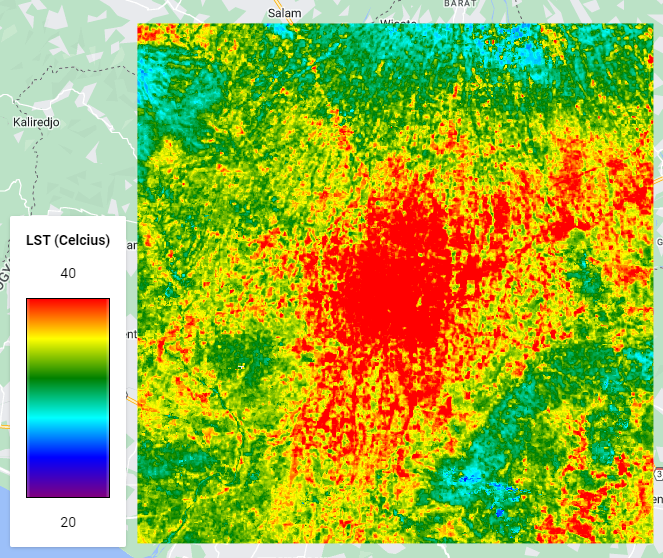
\includegraphics[width=40ex]{lst2023Truth.png}
	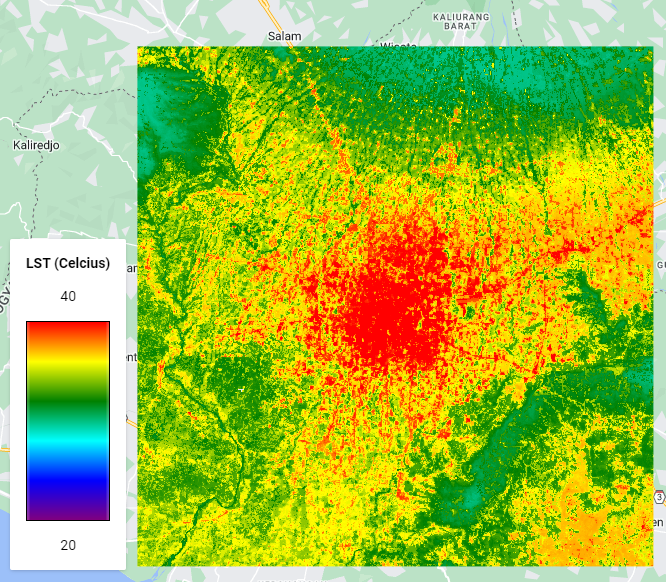
\includegraphics[width=40ex]{lst2023Prediction.png}
	\caption{Reference (left) and predicted (rigth) LST in 2023}
\end{figure}

\begin{figure}[htbp]
	\label{fig:r22023}
	\centering
	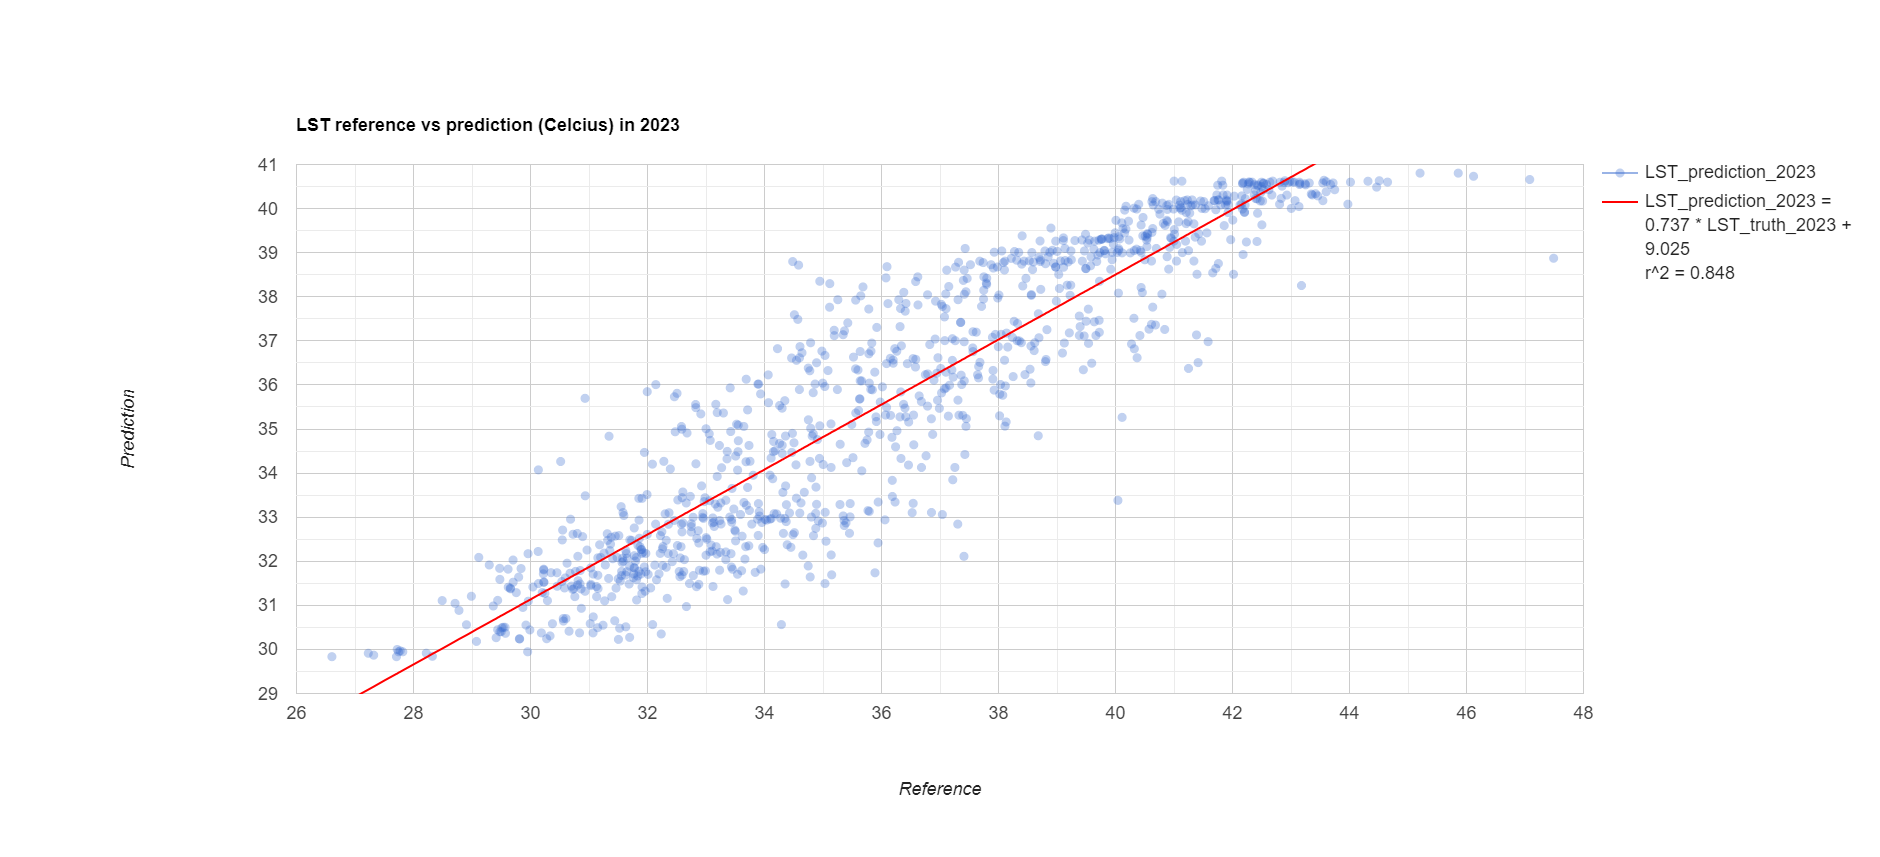
\includegraphics[width=90ex]{lst2023Accuracy.png}
	\caption{Accuracy assessment prediction for LST 2023}
\end{figure}
\printbibliography

\end{document}